\section{Case Studies}


\subsection{Controlled Studies I - Autoregressive Process} \label{sec:ar-study}


In our simulation exercise the performance of the QRAL model is evaluated by simulating data from an AR(1) model and then trying to recover its quantiles using QRAL and other competing models, namely:
\begin{enumerate}
\item \textbf{Quantile Regularized Adaptive LASSO (QRAL)} - estimates a different model for each quantile $Q_{y_t|X}(\alpha,\cdot)$, for all ${j \in J}$. In practice, this means that each coefficient $\beta_{1j}$ is estimated with regularization on each quantile. %As the QRAL estimates a different solution for all every $\alpha$-quantile of $y_t$, the model $$y_t^{\alpha_j} = \beta_{0\alpha_j} + \beta_{\alpha_j} y_{t-1}, \quad \text{for all } j \in J$$ will produce as output a different model for each probability quantile $y_t^{\alpha_j}$.
\item \textbf{Quantile Regression as Koenker (QRK)} - originally proposed by \cite{koenker1978regression}, where each coefficient $\beta_{1j}$ is estimated independently using QR. 
\item \textbf{Autoregressive (AR)} - a simple Gaussian model.

\end{enumerate}

The AR(1) specification is given by:
\begin{equation}
y_t = \beta_0 + \beta_1 y_{t-1} + \varepsilon_t, \quad \varepsilon_t \sim N(0, 1), \quad t=1,\dots,400 \label{eq:ar1}
\end{equation}
with $\beta_0 = 0$, $\beta_1 = 0.3$ and $y_0 = 0$. % This length is chosen because the sample size of the RG time series generally has such a size.

The interquantile regularization parameter $\gamma$ (see equations (\ref{eq:adaLASSO-1})-(\ref{eq:adaLASSO-ult})) is estimated using cross-validation, which is a popular technique for selecting the best value of parameters for cross-sectional data. 
Since in this experiment the model has only one lag, the model selection will not be evaluated, hence $\lambda=0$.
After simulating 1000 different time series given by equation (\ref{eq:ar1}), the three models are estimated.
% TODO referência cross-validation

Since the main objective of this simulation experiment is to evaluate how our nonparametric model can correctly recover the true AR(1) process, the model performance can be evaluated by examining how closely the estimated quantiles are from the populational ones. The results for each model are depicted in Figure \ref{fig:boxplot-ar1}, where a Boxplot containing the results for the 1000 simulations is shown. %a single boxplot for AR(1) and one for each probability $\alpha$ for QRAL and QRK.
\begin{figure}[ht]
	\centering
	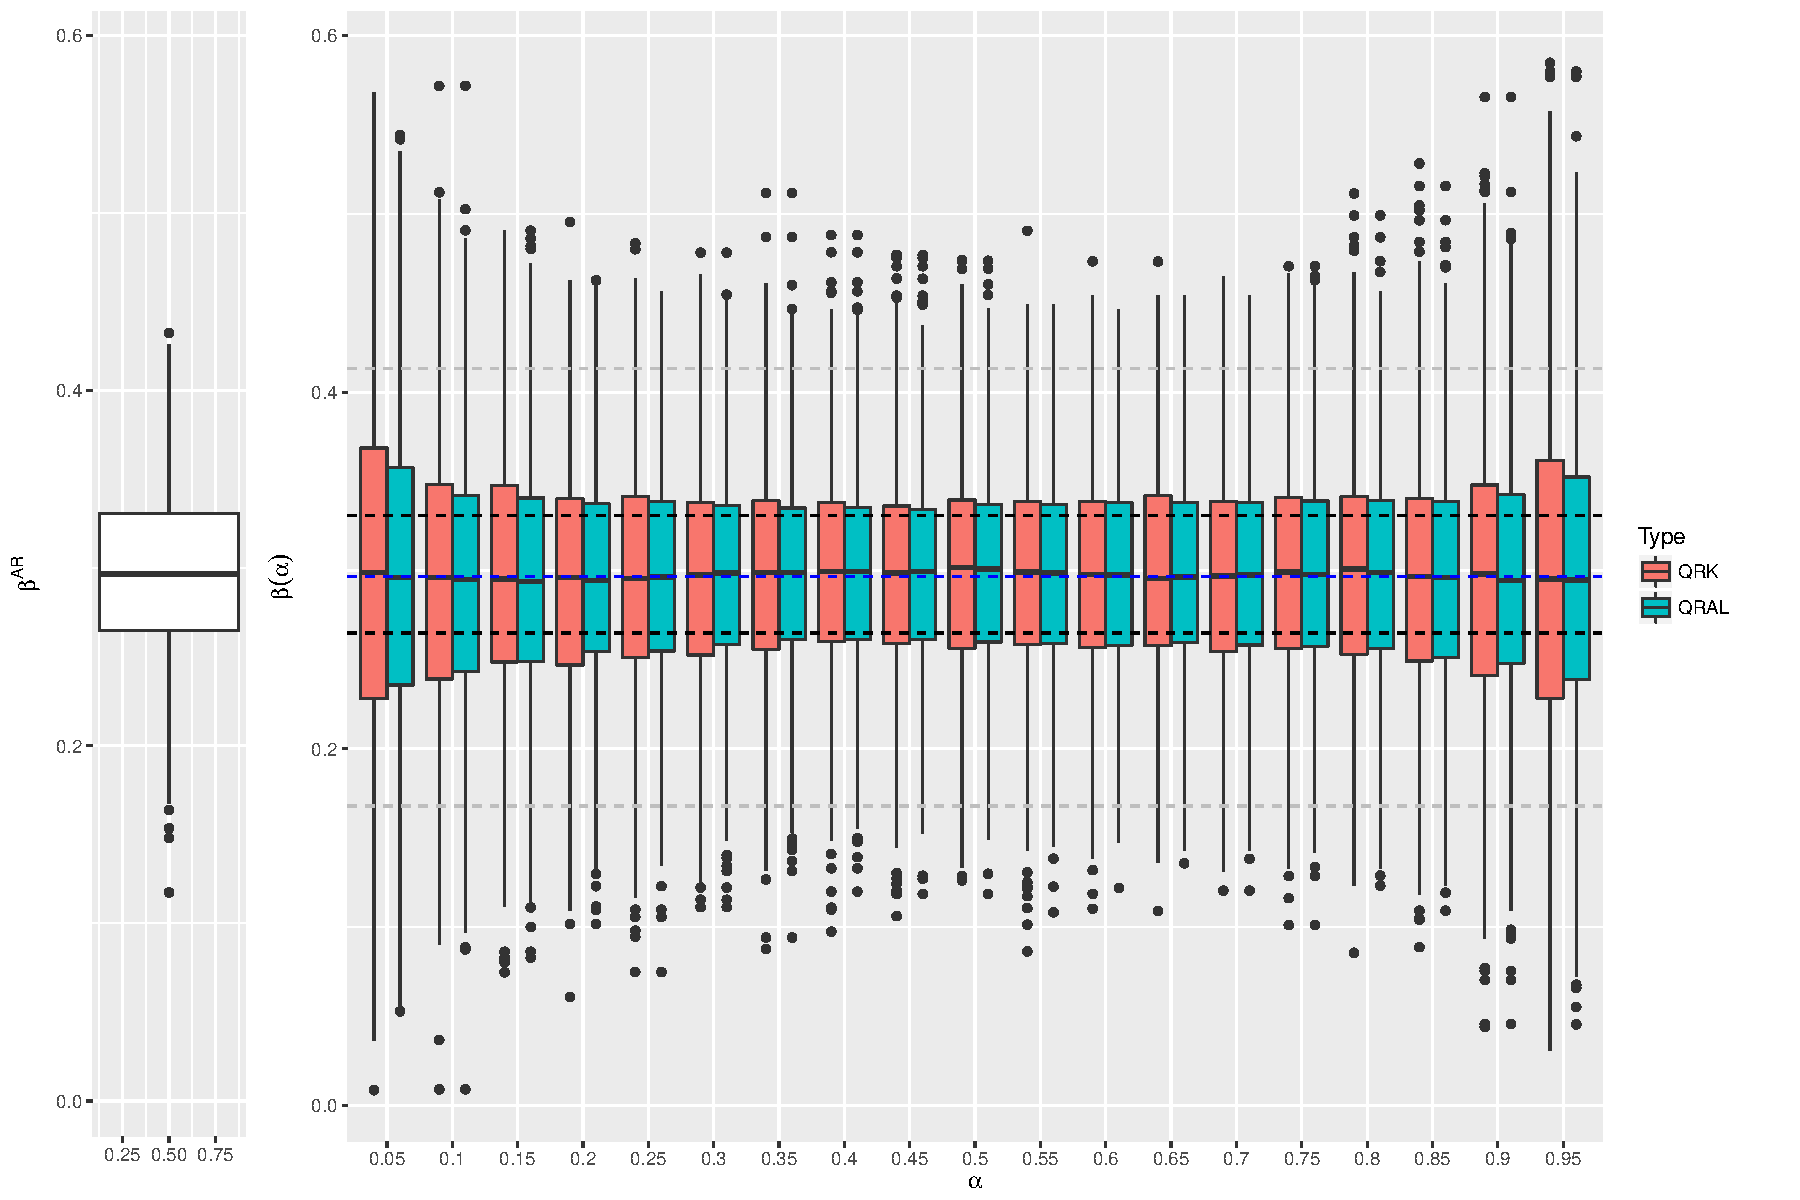
\includegraphics[width=1.0\linewidth]{Images/boxplot-ar1.pdf}
	\caption{Boxplot showing estimated coefficient after 1000 iterations. The boxplot of the AR(1) coefficient estimation is on the left hand side. Note that for the AR(1) the coefficient is equal for all probabilities $\alpha$. The boxplot of the regular QR (where $\gamma = 0$) and the QRAL where $\gamma$ is selected using cross-validation is on the right hand side }
	\label{fig:boxplot-ar1}
\end{figure}
The conclusions from this experiment are: (i) coefficient estimation errors for the central quantiles are not far from those estimated by the AR model; (ii) extreme quantiles are usually harder to estimate due to having fewer observations, and as a consequence the estimation error increases on the extremes; (iii) QRAL has an advantage over QRK by showing smaller variance of estimators.


\subsection{Case study with real data}


% Sobre o estudo de caso, Qd falar do que fez fala vc ajustou a métrica para minimizar o erro da previsão quantilica um passo à frente, como é de costume na literatura.  Para ilustrar a metodologia, vc tb ajustou os parâmetros de regularização com base na performance média para 4 passos à frente. Daí vc usa a parte que tá lá de que vc usou a simulação. Veja se K está definido. Senti falta no paper de ter o K. Se não tiver, talvez seja melhor não definir... vc só fala 4 passos à frente... aguardo próxima vs. 



In this section, the QRAL methodology is tested in generating future scenarios for a real RG time series. The wind power time series, measured in megawatts, is composed of 2 years (from June-2011 to May-2013) of hourly power generation observations from a wind farm located in the Brazilian Northeast. % Figure \ref{fig:icaraizinho-mensal} depicts a time series plot from which a strong seasonal pattern can be seen. 
% The annual seasonality is seen in Figure \ref{fig:icaraizinho-mensal}, where each individual year is plotted as a single line on the graph. 
% \begin{figure}[ht]
% \centering
% 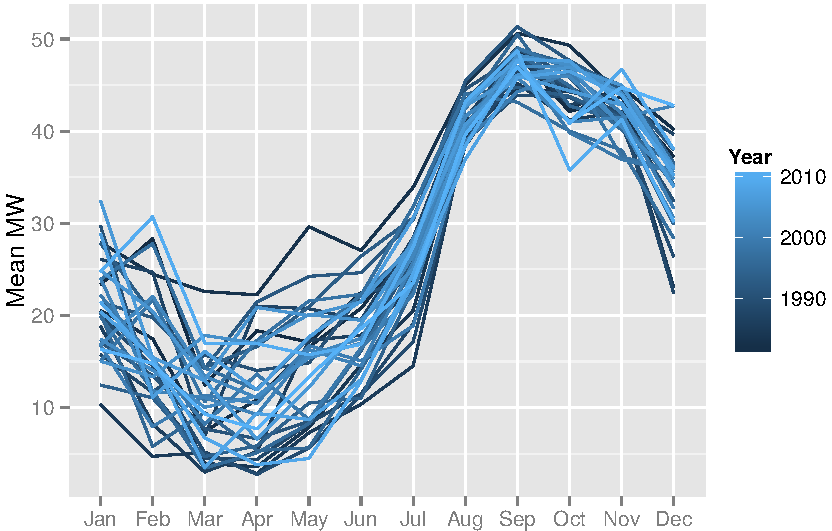
\includegraphics[width=0.8\linewidth]{Images/icaraizinho-mensal2.pdf}
% \caption{Icaraizinho annual data. Each series consists of monthly observations for each year.}
% \label{fig:icaraizinho-mensal}
% \end{figure}

As previously mentioned on section \ref{sec:estimation-evaluation-simulation}, the case study is evaluated using a rolling window scheme. At each step, the model is estimated over a window of size 720 (corresponding to a month worth of hourly observations) and the quantiles of the next $K$ periods are forecasted. The rolling window estimation is repeated for 500 consecutive times, each of which are consisted by $K$ periods ahead forecast.
Concerning the QRAL model, the parameters $\lambda$ and $\gamma$ are kept the same across all dataset. These regularization parameters are selected among a thin grid of values according to two metrics: MAE and SIC.

We use four different models to generate scenarios for hourly wind power time series:  QRAL, QRK, QRL (Quantile Regularized LASSO is essentially the same model as QRAL in which we let $w_{ij} = 1$ for all $i$ and $j$) and SARIMA. 
The tuning parameters $\lambda$ and $\gamma$ of QRL and QRAL are selected according to the two metrics presented in Section \ref{sec:estimation-evaluation-simulation}: SIC and MAE.
We estimate the SARIMA model using the \emph{forecast} \cite{hyndman2008forecastpackage} package from R, via the \emph{auto.arima} function, which selects the best model according to an IC (details in \cite{hyndman2008forecastmanual}).


The resulting tuning parameters estimates followed by SIC and MAE metric values for all models is shown in Table \ref{tab:results-icaraizinho}. We tested our model against the benchmarks for the one-step ahead forecasting, as it is typical in the literature, and for the four-step ahead. The parameters $\lambda$ and $\gamma$ may differ for each different horizon, as they are chosen in order to be the best model according to the criteria and horizon it is being built for. The forecasted quantiles from the QRAL model are directly evaluated against the historic data on the one-step ahead case. On the other hand, when forecasting four steps ahead, we use Algorithm \ref{alg:mc-procedure} in order to simulate future quantiles.
In all metrics and horizons, the performance of QRAL is superior to QRL. In both horizons, the scenarios providaded by QRAL (MAE) have the smallest forecasted errors according to metric MAE, which suggests it is a model capable of handling better asymmetric data than a model such as SARIMA. The choice of SIC appears not to be a good strategy when the goal is to maximize forecasting performance across many quantiles. The models chosen by this criteria, in our experiment, did not find regularization parameters that were also good in forecasting quantiles.
\begin{table}[]
	\centering
	\caption{Cumulated statistics across all $\alpha_j$ quantiles}
	\label{tab:results-icaraizinho}	
	\begin{tabular}{llllll}
		\hline
		Method (tuning criteria) & Horizon     & $\lambda$     & $\gamma$     & SIC            & MAE             \\ \hline
		QRL (SIC)                & 1h          & 2.7           & 0            & 7.13           & 1.99\%          \\
		QRL (MAE)                & 1h          & 17            & 0            & 8.4            & 1.61\%          \\
		\textbf{QRAL (SIC)}      & \textbf{1h} & \textbf{1}    & \textbf{0}   & \textbf{7.09}  & \textbf{2.04\%} \\
		\textbf{QRAL (MAE)}      & \textbf{1h} & \textbf{20}   & \textbf{1.0} & \textbf{8.39}  & \textbf{0.98\%} \\
		QRK                      & 1h          & 0             & 0            & 8.34           & 3.50\%          \\
		SARIMA                   & 1h          & -             & -            & -              & 2.10\%          \\ \hline
		QRL (SIC)                & 4h          & 2.3           & 0            & 13.23          & 2.40\%          \\
		QRL (MAE)                & 4h          & 0             & 0            & 13.73          & 2.10\%          \\
		\textbf{QRAL (SIC)}      & \textbf{4h} & \textbf{2.5}  & \textbf{0}   & \textbf{13.16} & \textbf{2.03\%} \\
		\textbf{QRAL (MAE)}      & \textbf{4h} & \textbf{6.75} & \textbf{7.0} & \textbf{13.3}  & \textbf{1.64\%} \\
		QRK                      & 4h          & 0             & 0            & 13.73          & 2.10\%          \\
		SARIMA                   & 4h          & -             & -            & -              &     3.26\%            \\ \hline
		\end{tabular}
\end{table}


One of the main objectives of this work is generating future scenarios, so in the sequence we further investigate the case with horizon four. Figure \ref{fig:heatmap-qral-mae} presents a heatmap of the MAE metric for the QRAL model for a combination of regularization parameters. We see that there is a region of optimal levels of regularization according to this criteria. The worst performances occurs when $\lambda = 0$, such that all covariates are included in the model.
\begin{figure}[ht]
	\centering
	\includegraphics[width=1.0\linewidth]{Images/QRAL-MAE-4h.pdf}
	\caption{Calculated MAE of forecasting quantiles in a 4 hour window. Lower values have a lighter tone, while higher ones are darker.}
	\label{fig:heatmap-qral-mae}
\end{figure}


Since coefficients are estimated using a rolling window scheme, they are refreshed at each step. As their regularization parameters are kept constant, the figures of a given period is sufficient  to understand the coefficients behaviour in the experiment as a whole. Figures \ref{fig:betas-qrk} and \ref{fig:betas-MAE} present the estimated coefficients for the QRAL (MAE) and the QRK on the first period of the experiment, respectively.
\begin{figure}
	\centering
	\includegraphics[width=1.0\linewidth]{Images/Plot_betas-QRK.pdf}
	\caption{Estimated coefficients for the QRK model at time $t =1$.}
	\label{fig:betas-qrk}
\end{figure}
\begin{figure}
	\centering
	\includegraphics[width=1.0\linewidth]{Images/Plot_betas-QRAL-MAE-4h.pdf}
	\caption{Estimated coefficients for the QRAL (MAE) model at time $t =1$.}
	\label{fig:betas-MAE}
\end{figure}
For each of these models, $\beta_0(\alpha)$ is shown on the left hand side of the figure, while $\beta(\alpha)$, for each lag, is on the right side. 
A comparison of coefficients between QRAL (MAE) and QRK ilustrates clearly the effect of regularization, as the QRAL is essentially the QRK model with regularization on both variable selection (via LASSO) and interquantile (via the second derivative penalization). 
One advantage of the proposed model is that quantiles are jointly estimated in a single model, which helps to decrease the variance of the estimators. As a consequence, only a handful of coefficients are selected to be nonzero, and its $\beta$ coefficients are regularized piecewise linear functions, in contrast to QRK's noisier and with higher variability coefficients (as seen in the experiment in section \ref{sec:ar-study}). 

In Figures \ref{fig:scenarios-qral}-\ref{fig:scenarios-sarima}, we compare the median (50\%), extreme quantiles (5\% and 95\%) and the 1st and 3rd quartiles (25\% and 75\%) obtained from QRAL (MAE), QRK and SARIMA models via simulation with the associated historic time series. As an advantage of QR models is the fact that they are able to capture an asymmetric non Gaussian distribution, which a SARIMA model cannot.  
\begin{figure}[ht]
	\centering
	\includegraphics[width=1.0\linewidth]{Images/Plot_scenarios-QRAL-MAE-4h.pdf}
	\caption{Comparison of real data with generated scenarios using QRAL (MAE). The scenarios are generated at the period of each red dot in the plot, with a 4 hours horizon. }
	\label{fig:scenarios-qral}
\end{figure}
\begin{figure}[ht]
	\centering
	\includegraphics[width=1.0\linewidth]{Images/Plot_scenarios-QRK.pdf}
	\caption{Comparison of real data with generated scenarios using QRK. The scenarios are generated at the period of each red dot in the plot, with a 4 hours horizon.}
	\label{fig:scenarios-qrk}
\end{figure}
\begin{figure}[h]
	\centering
	\includegraphics[width=1.0\linewidth]{Images/Plot_scenarios-SARIMA.pdf}
	\caption{Comparison of real data with generated scenarios using SARIMA. The scenarios are generated at the period of each red dot in the plot, with a 4 hours horizon.}
	\label{fig:scenarios-sarima}
\end{figure}


